\section{Spécifications}

\subsection{Caractérisation de l'environement}

L'environnement du circuit est constitué de deux entités :
\\

L'ensemble « \textbf{Système à uP} » formé par le processeur, le contrôleur mémoire et le
contrôleur d'interruptions ;
\\

Un \textbf{esclave I2C} distant (capteur, mémoire, etc.).
\\

L'entité Système à uP peut configurer le contrôleur, écrire l'adresse de l'esclave, écrire les
données à envoyer, lancer une transaction, lire l'état, lire les données reçues et gérer
l'interruption produite. L'entité Esclave distant répond à son adresse, acquitte les octets
reçus, ou émet des octets lorsque le maître lit.
\\

Comportement de l'entité Système à uP (en considérant les cycles de fonctionnement
comme instantanés) : depuis l'état Autre, le processeur évolue selon les événements
suivants :
\\

\begin{figure}[H]
    \centering
    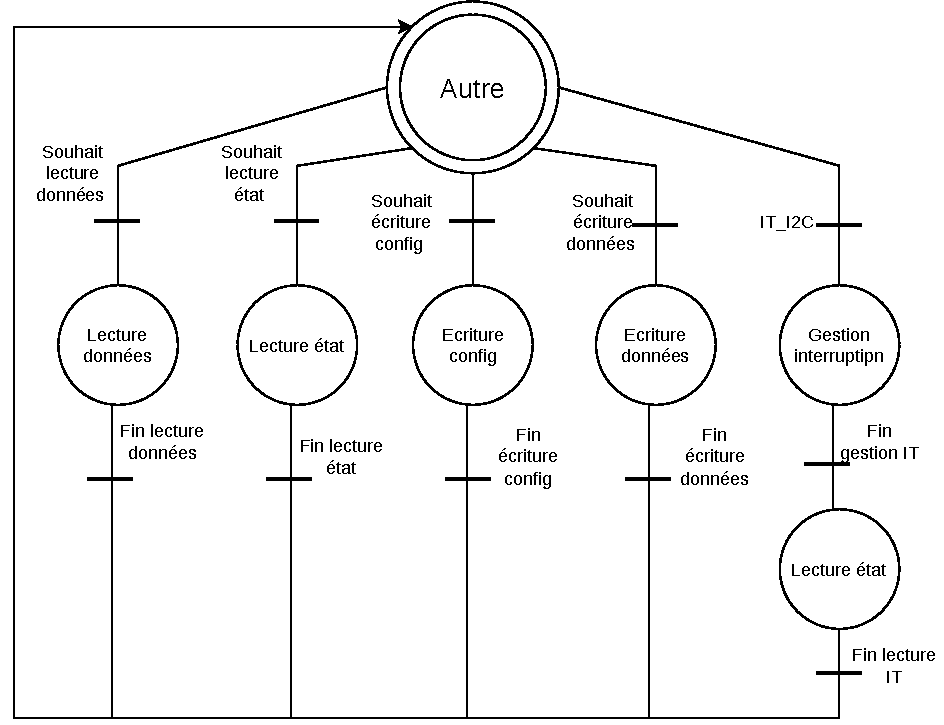
\includegraphics[width=0.95\linewidth]{Images/2_SPEC/Comportement_uc.pdf}
    \caption{Comportement de l'entité Système à uP}
\end{figure}